\documentclass[a4paper, 11pt]{article}
\usepackage{geometry}
\usepackage{indentfirst}
\usepackage{setspace}
\usepackage{amsmath}
\usepackage{graphicx}
\usepackage{wrapfig}
\usepackage{caption}
\usepackage{indentfirst}
\setlength{\parindent}{20pt}
\usepackage{amssymb}
\usepackage{float}

\graphicspath{ {./images/} }
\geometry{left=2.5cm, right=2.5cm, top=2.5cm, bottom=2.5cm}

\begin{document}	
	\title{Exercise \# 2. Iterative Methods For Linear Systems. }
	\author{{\small Alexandre Rodrigues (2039952)}}
	\date{\today}
	
	\maketitle
		\section*{Question 1}
			Using as a test the example usage, with $tol = 1 \times 10^{-8}$ and limiting the iterations to $maxit=250$ I got the following results. 
		
			\begin{figure}[H]
				\centering
				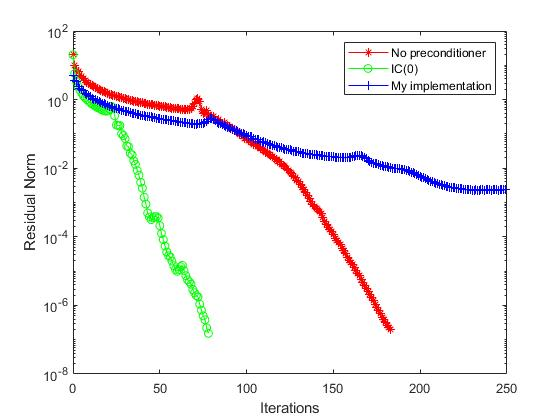
\includegraphics[width=.6\linewidth]{ex1_it250.jpg}
				\caption{Residual norm vs iteration number for PCG methods, $maxit=250$}
				\label{fig:ex1_it250}
			\end{figure}
		
			\begin{table}[H]
				\centering
				\begin{tabular}{c|c|c|c}
					\textbf{Method} 					&  \textbf{Iterations} 	& \textbf{Final Residual} 		& \textbf{Computational Time} 	\\ \hline
					Matlab PCG without preconditioning	& 			$183$ 		& $ 1.9591 \times 10^{-7} $ 	& $ 0.077 s $					\\ \hline
					Matlab PCG IC(0)					& 			$78$ 		& $ 1.5293 \times 10^{-7} $ 	& $ 0.068 s $					\\ \hline	
					My PCG implementation				& 			$250$		& $ 2.3 \times 10^{-3} $		& $	0.151 s $					\\
				\end{tabular}
				\caption{Results of PCG methods, $maxit=250$}
				\label{table:ex1_it250}
			\end{table}
		
			When $ maxit $ is large enough to guarantee convergence in all implementations we get the following results:
			\begin{figure}[H]
				\centering
				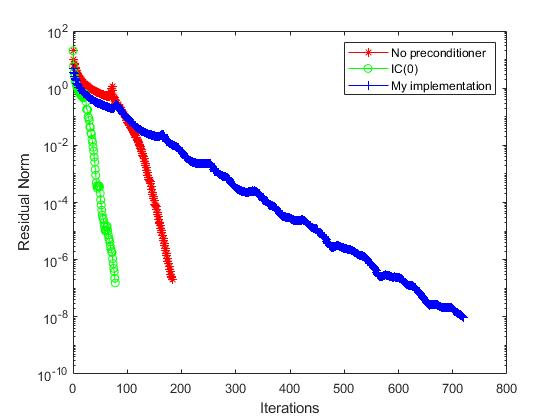
\includegraphics[width=.6\linewidth]{ex1_it750.jpg}
				\caption{Residual norm vs iteration number for PCG methods, $maxit=750$}
				\label{fig:ex1_it750}
			\end{figure}
		
			\begin{table}[H]
				\centering
				\begin{tabular}{c|c|c|c}
					\textbf{Method} 					&  \textbf{Iterations} 	& \textbf{Final Residual} 		& \textbf{Computational Time} 	\\ \hline
					Matlab PCG without preconditioning	& 			$183$ 		& $ 1.9591 \times 10^{-7} $ 	& $ 0.054 s $					\\ \hline
					Matlab PCG IC(0)					& 			$78$ 		& $ 1.5293 \times 10^{-7} $ 	& $ 0.063 s $					\\ \hline	
					My PCG implementation				& 			$720$		& $ 9.6833 \times 10^{-9} $		& $	0.351 s $					\\
				\end{tabular}
				\caption{Results of PCG methods, $maxit=750$}
				\label{table:ex1_it750}
			\end{table}
			
			My implementation is slower to converge but produces better final residual values.
			
			
		\section*{Question 2}
			The spectral condition number of A is 
			
			\begin{equation}
				\kappa(A) = \frac{\lambda_{max}(A)}{\lambda_{min}(A)}.
			\end{equation}
		
			In Matlab I used the \texttt{condest(A)} function to estimate the condition number of a sparse matrix A.
		
			\begin{table}[H]
				\centering
				\begin{tabular}{c|c|c|c|c|c|c|c}
					$n_x$   & $ h $						& $\kappa(A)$			 & $ \sqrt{\kappa(A)} $& $ CG $ & $ PCG(0) $& $PCG(10^{-2})$& $PCG(10^{-3})$ \\ \hline
					$ 102 $ & $ 1.0000 \times 10^{-4} $ & $ 6.0107 \times 10^3 $ & $ 77.5288 $ 		& $ 283 $ 	& $ 87 $ 	& $ 45 $ 		& $ 17 $ 		\\ \hline
					$ 202 $ & $ 2.5000 \times 10^{-5} $ & $ 2.3810 \times 10^4 $ & $ 154.3039 $ 	& $ 532 $ 	& $ 159 $ 	& $ 78 $ 		& $ 30 $ 		\\ \hline
					$ 402 $ & $ 6.2500 \times 10^{-6} $ & $ 9.4770 \times 10^4 $ & $ 307.8473 $ 	& $ 948 $ 	& $ 282 $ 	& $ 137 $ 		& $ 53 $		\\ \hline
					$ 802 $ & $ 1.5625 \times 10^{-6} $ & $ 3.7814 \times 10^5 $ & $ 614.9304 $ 	& $ 1792 $	& $ 533 $ 	& $ 258 $ 		& $ 97 $ 		\\ 
				\end{tabular}
				\caption{Iterations of PCG methods for each value of $n_x$ and respective values of $h$ and $\kappa(A)$}
				\label{table:ex2}
			\end{table}	
		
			One can note from the table the dependence of the number of iterations on $ h = \frac{1}{N} = \frac{1}{(nx-2)^2} $.
			The number of iterations is halved when $n_x$ approximately doubles.		
			
				
		\section*{Question 3}
			show theoretically ??
			
			When using the Choledsky precontionier with no fill in, I did'nt get the expected results.
			Both Matlab's and my implementation converged in only one iteration.
			
			\begin{figure}[H]
				\centering
				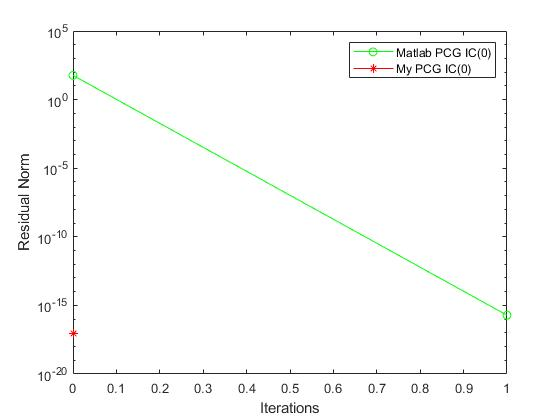
\includegraphics[width=.6\linewidth]{ex3.jpg}
				\caption{Residual norm vs iteration number for PCG methods with $IC(0)$ preconditioner}
				\label{fig:ex3}
			\end{figure}
		
			
			Due to the bad results, I tried to remove preconditioning form my implementation by setting $L$ as the identity matrix, \texttt{L = speye(size(L))}.
			\begin{figure}[H]
					\centering
					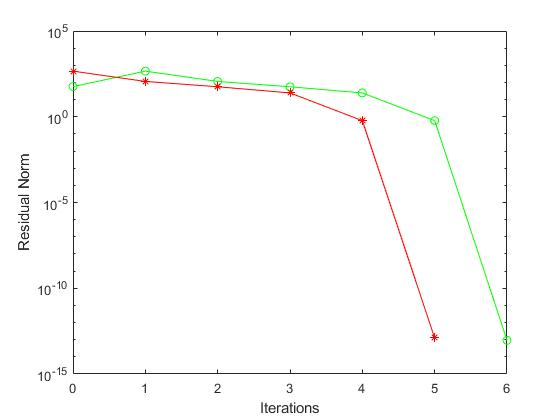
\includegraphics[width=.6\linewidth]{ex3_NoPrec.jpg}
					\caption{Residual norm vs iteration number for PCG methods without preconditioning}
					\label{fig:ex3_NoPrec}
			\end{figure}
		
			\begin{table}[H]
				\centering
				\begin{tabular}{c|c|c|c}
					\textbf{Method} &  \textbf{Iterations} 	& \textbf{Final Residual} 		& \textbf{Computational Time} 	\\ \hline
					Matlab PCG		& 			$6$ 		& $ 9.2128 \times 10^{-14} $ 	& $ 0.021 s $	\\ \hline	
					My PCG 			& 			$5$			& $ 1.2744 \times 10^{-13} $	& $	0.012 s $	\\ \hline
				\end{tabular}
				\caption{Results for each value of implementation, no preconditioning}
				\label{table:ex3_NoPrec}
			\end{table}
			These results show the theoretical calculations, my implementation is still better than expected.
			
		
		
		
		\section*{Question 4}		
			\begin{figure}[H]
				\centering
				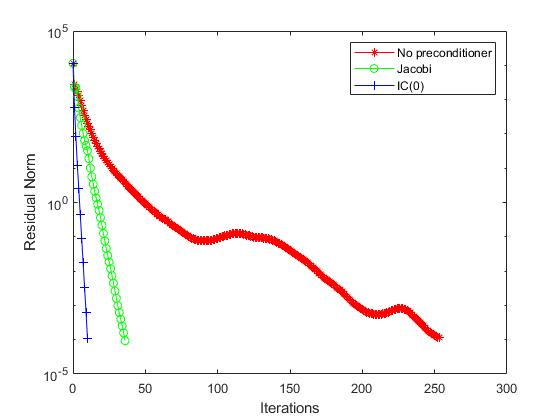
\includegraphics[width=.6\linewidth]{ex4.jpg}
				\caption{Residual norm vs iteration number for PCG methods without preconditioning}
				\label{fig:ex4}
			\end{figure}
		
			\begin{table}[H]
			\centering
			\begin{tabular}{c|c|c|c}
				\textbf{Preconditioner} &  \textbf{Iterations} 	& \textbf{Final Residual} 		& \textbf{Computational Time} 	\\ \hline
				None					& 			$253$ 		& $ 1.1367 \times 10^{-4} $ 	& $ 0.254 s $	\\ \hline
				Jacobi					& 			$36$ 		& $ 9.3198 \times 10^{-5} $ 	& $ 0.053 s $	\\ \hline		
				IC(0)					& 			$10$		& $ 1.1155 \times 10^{-4} $		& $	0.046 s $	\\
			\end{tabular}
			\caption{Results for each preconditioner}
			\label{table:ex4}
			\end{table}
		
			There is a very clear improvement when using preconditioning.
			It is also noticeable the superior characteristics of the incomplete Choledsky preconditioner relative to Jacobi.
		
		\section*{Question 5}
			\begin{figure}[H]
				\centering
				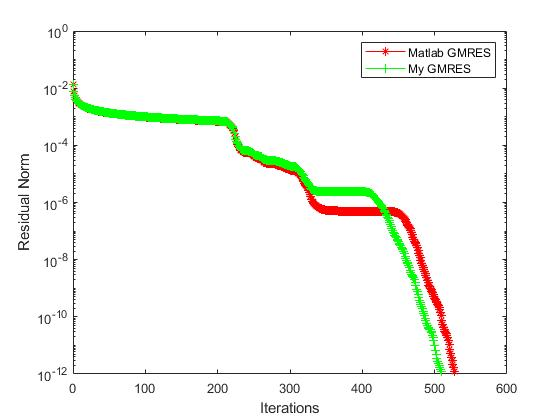
\includegraphics[width=.6\linewidth]{ex5.jpg}
				\caption{Residual norm vs iteration number for GMRES methods}
				\label{fig:ex5}
			\end{figure}
		
			\begin{table}[H]
				\centering
				\begin{tabular}{c|c|c|c}
					\textbf{Method} &  \textbf{Iterations} 	& \textbf{Final Residual} 		& \textbf{Computational Time} 	\\ \hline
					Matlab GMRES	& 			$527$ 		& $ 1.2073 \times 10^{-12} $ 	& $ 9.097 s $	\\ \hline
					My GMRES		& 			$509$ 		& $ 1.2231 \times 10^{-12} $ 	& $ 10.032 s $	\\ 
				\end{tabular}
				\caption{Results for each GMRES implementation}
				\label{table:ex5}
			\end{table}
			
			These results show that the methods have very similar convergence characteristics.
			My implementation has a smaller number of iterations but the other results are slightly worse than the ones achieved with Matlab's implementation.
			
		
		\section*{Question 6}
			\begin{figure}[H]
				\centering
				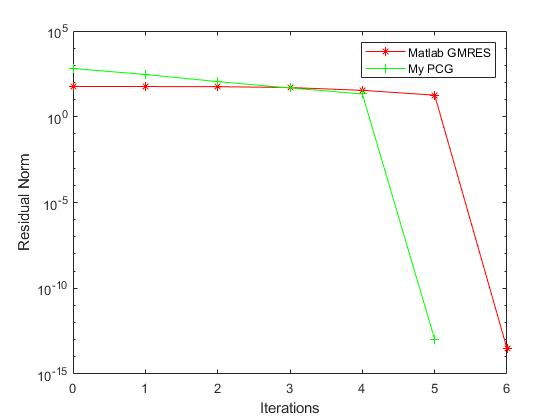
\includegraphics[width=.6\linewidth]{ex6.jpg}
				\caption{Residual norm vs iteration number for preconditioned GMRES methods}
				\label{fig:ex6}
			\end{figure}
			
			\begin{table}[H]
				\centering
				\begin{tabular}{c|c|c|c|c}
					\textbf{Method} &  \textbf{Iterations} 	& \textbf{Final Residual} 	 & \textbf{True Residual}		& \textbf{Computational Time} 	\\ \hline
					Matlab GMRES	& 			$38$ 		& $ 1.5592 \times 10^{-10} $ & $ 4.5350 \times 10^{-13} $	& $ 0.121 s $	\\ \hline
					My GMRES		& 			$39$ 		& $ 2.3797 \times 10^{-13} $ & $ 7.1893 \times 10^{-14} $	& $ 4.943 s $	\\ 
				\end{tabular}
				\caption{Results for each preconditioned GMRES implementation}
				\label{table:ex6}
			\end{table}
			
			There are clear differences in the residuals and computation time values.
			My implementation is 40 times slower but produces a true residual 5 times smaller.		
		
		
		Solving the linear system in 3b produced the same unexpected results as in that question.
		When using the Choledsky precontionier with no fill in both Matlab's and my implementation converged in only one iteration.
		
		\begin{table}[H]
			\centering
			\begin{tabular}{c|c|c|c}
				\textbf{Method} &  \textbf{Iterations} 	& \textbf{Final Residual} 		& \textbf{Computational Time} 	\\ \hline
				GMRES 			& 			1 			& $ 3.8481 \times 10^{-16} $	& $ 0.027 s $	\\ \hline	
				My PCG 			& 			1			& $ 1.7554 \times 10^{-17} $	& $ 0.003 s $	\\ \hline
			\end{tabular}
			\caption{Iterations for each value of nx}
			\label{table:ex6_c_prec}
		\end{table}	
	
		When I removed preconditioning form my implementation by setting $L$ as the identity matrix, \texttt{L = speye(size(L))}.
			
		\begin{table}[H]
			\centering
			\begin{tabular}{c|c|c|c}
				\textbf{Method} &  \textbf{Iterations} 	& \textbf{Final Residual} 		& \textbf{Computational Time} 	\\ \hline
				GMRES			& 			$6$ 		& $ 3.0413 \times 10^{-14} $ 	& $ 0.102 s $	\\ \hline	
				My PCG 			& 			$5$			& $ 1.0468 \times 10^{-13} $	& $ 0.012 s $	\\ \hline
			\end{tabular}
			\caption{Results for each value of implementation, no preconditioning}
			\label{table:ex6_c_NoPrec}
		\end{table}
	
		\begin{figure}[H]
			\centering
			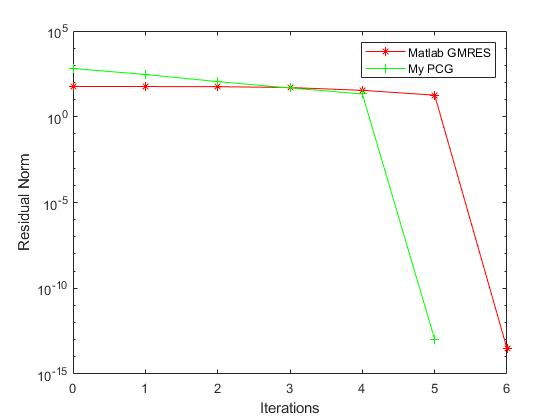
\includegraphics[width=.6\linewidth]{ex6b.jpg}
			\caption{Residual norm vs iteration number for GMRES methods without preconditioning}
			\label{fig:ex6_c_NoPrec}
		\end{figure}
	
		As in 3b, these results show the theoretical calculations, my implementation is still better than expected.
		
		
		
		\section*{Question 7}
		
			\begin{table}[H]
				\centering
				\begin{tabular}{c|c|c|c}
					\texttt{\textbf{restart}} &  \textbf{Iterations} 	& \textbf{Final Residual} 		& \textbf{Computational Time} 	\\ \hline
					$ 10 $			& 			$1149$ 		& $ 1.9901 \times 10^{-12} $ 	& $ 1.735 s $	\\ \hline	
					$ 20 $			& 			$739$		& $ 1.9741 \times 10^{-12} $	& $ 1.443 s $	\\ \hline
					$ 30 $			& 			$88$ 		& $ 1.3800 \times 10^{-12} $ 	& $ 0.242 s $	\\ \hline	
					$ 50 $			& 			$41$		& $ 9.9416 \times 10^{-13} $	& $ 0.135 s $	\\ \hline
				\end{tabular}
				\caption{Results for each value of \texttt{restart}}
				\label{table:ex7}
			\end{table}
			
			\begin{figure}[H]
				\centering
				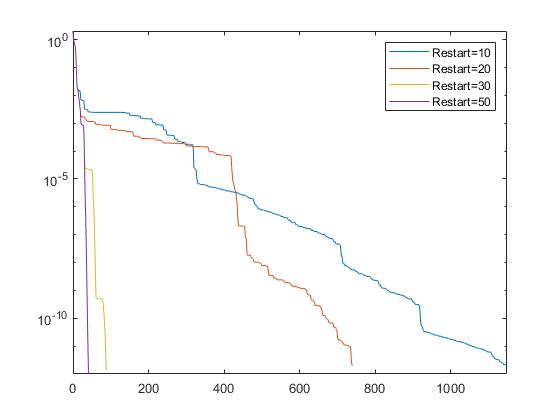
\includegraphics[width=.6\linewidth]{ex7.jpg}
				\caption{Residual norm vs iteration number for each value of \texttt{restart}}
				\label{fig:ex7}
			\end{figure}
			
			One can notice a clear improvement in convergence with the increase of the \texttt{restart} value.
			$\ldots$
		
		\section*{Question 8}
		
			Using \texttt{maxit=550}, \texttt{tol=1e-8}$\ldots$
			
			\begin{table}[H]
				\centering
				\begin{tabular}{c|c|c|c|c|c|c}
					\textbf{Tolerance} & \textbf{Iterations} & \textbf{Prec. Time}  & \textbf{Tsol}  & \textbf{Ttotal} & \textbf{Final Residual} & \textbf{$ \rho $} \\ \hline
					$2 \times 10^{-2}$ & $1316$	& $ 37.92 s $ 	& $ 44.53 s $ & $ 82.45 s $ 	& $ 5.2065 \times 10^{-7} $ & $ 0.4537 $\\ \hline
					$1 \times 10^{-2}$ & $4444$	& $ 40.55 s $ 	& $ 22.86 s $ & $ 63.42 s $ 	& $ 5.7213 \times 10^{-7} $ & $ 0.5807 $\\ \hline
					$3 \times 10^{-3}$ & $150$	& $ 51.78 s $ 	& $ 7.39 s $ & $ 59.17 s $ 		& $ 6.4998 \times 10^{-7} $ & $ 0.9401 $\\ \hline
					$1 \times 10^{-3}$ & $67$	& $ 47.74 s $ 	& $ 3.63 s $ & $ 51.37 s $ 		& $ 8.5337 \times 10^{-7} $ & $ 1.4544 $\\ \hline
					$1 \times 10^{-4}$ & $26$	& $ 43.30 s $ 	& $ 2.30 s $ & $ 45.60 s $ 		& $ 9.1517 \times 10^{-7} $ & $ 3.5140 $\\ \hline
					$1 \times 10^{-5}$ & $12$	& $ 96.73 s $ 	& $ 2.69 s $ & $ 99.42 s $ 		& $ 9.4359 \times 10^{-7} $ & $ 9.0720 $\\ \hline
				\end{tabular}
				\caption{Results for each value of tolerance}
				\label{table:ex8}
			\end{table}
			
			\begin{figure}[H]
				\centering
				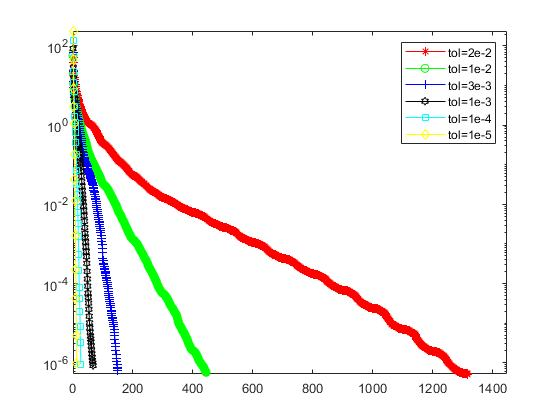
\includegraphics[width=.6\linewidth]{ex8.jpg}
				\caption{Residual norm vs iteration number for each value of tolerance}
				\label{fig:ex8}
			\end{figure}
	
\end{document}



